\section{Data}\label{sec:data}

All data are public. Table~\ref{tab:sources} in Appendix~\ref{app:repro} lists the sources
and their licences; the repository records the retrieval date and checksum of every file.

\subsection{The Thai CPI}

The Thai consumer price index is compiled monthly by the Trade Policy and Strategy Office
(TPSO) of the Ministry of Commerce. The current base year is 2566 in the Buddhist era (2023),
and the series on this base has been in use since January 2568 (2025)
\citep{tpso2025cpinote}. Like most national CPIs it is a Lowe index
\citep{imf2020cpimanual}: expenditure weights from a base period, price-updated to a price
reference month, here December 2567. TPSO's open API publishes monthly indices for the
headline, divisions, groups and items \citep{tpso2026api}. It publishes no weights. The
monthly release publishes price-updated weight shares for the official aggregates only
(headline, the divisions, the food groups and the analytical series such as core CPI). We
recover those shares from the releases and check that they add up the hierarchy and
reproduce the official headline from the published sub-indices.

Below the published aggregates, item weights are not public. We partition the item codes
into \emph{cells}: each official aggregate owns the items whose deepest published ancestor it
is, and the cell weight is the aggregate's weight minus that of the published aggregates
nested below it. Within a cell we estimate item weights in two ways and report both: an equal
split (primary) and non-negative least squares on the Lowe identity, which chooses the split
that best reproduces the cell's index from its items' indices (sensitivity). Neither is an
official weight, and the paper never calls it one.

\subsection{Scope: the items a product classifier can reach}

A classifier of packaged-product text can only measure items sold as packaged products. We
define \NLabelsInScope{} in-scope CPI items: food at home, ready-to-eat food, non-alcoholic
beverages, alcoholic beverages, tobacco, personal care and cleaning products. Each is mapped
to its COICOP 2018 class \citep{unsd2018coicop}. Everything else (rents, energy, transport,
services, clothing, durable goods) is out of scope (\textsc{oos}). In-scope items carry
\InScopeWeightEqual\% of the headline weight under the equal split and \InScopeWeightNnls\%
under NNLS, most of it food (Figure~\ref{fig:coverage}).

\begin{figure}[t]
\centering
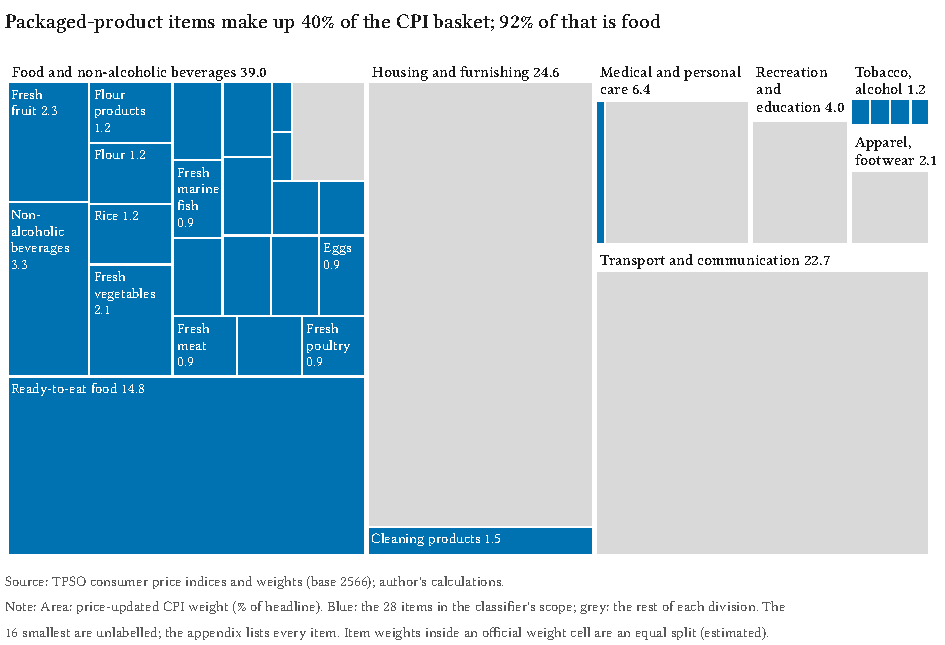
\includegraphics[width=\textwidth]{fig02_coverage.pdf}
\caption{\textbf{Packaged-product items are a large share of the Thai CPI basket, and most of
it is food.} Area: price-updated CPI weight (\% of headline), by division; blue, the
in-scope items; grey, the rest of each division. Item weights inside an official weight cell
are an equal split (estimated). Source: TPSO; author's calculations.}
\label{fig:coverage}
\end{figure}

\subsection{Product text}

\paragraph{Open Food Facts.} Open Food Facts (OFF) is a crowd-sourced, openly licensed
database of packaged products \citep{off2026}. We use its Parquet export and that of its
sister project Open Beauty Facts. Our extract holds \NOffProducts{} products from
\NOffMarkets{} markets: Thailand, other Asian markets and a sample of European products.
Of the \NOffThailand{} products tagged as sold in Thailand, \NOffThailandThaiScript{} have a
name in Thai script. Model input is the product's name, brand and quantity, joined as
\texttt{name | brand | quantity}.

\paragraph{Weak labels.} OFF products carry crowd-sourced category tags. A hand-curated
crosswalk maps tags to CPI items, following TPSO's own item headings rather than intuition
about COICOP (for example, snacks belong to flour products in the Thai CPI). This gives weak
labels: \NWeakNonthai{} non-Thai products and \NWeakThai{} Thai products. Weak labels are
used for training and development, never for evaluation.

\paragraph{Official specifications.} The Ministry of Commerce publishes the product
specifications TPSO uses for price collection: short Thai descriptions with brand and pack
size, each under an official item code \citep{moc2026specs}. These give \NMocSpecs{}
official labels. They are not shop listings, but they are the closest public analogue of
labelled Thai product text. We split them by item code, so that specifications of one item
never straddle training and test: \NMocTrainval{} for training and validation, \NMocTest{}
for test.

\subsection{Gold labels}\label{sec:gold}

Evaluation uses a gold sample of Thai OFF products labelled by the author. The frame is the
\NOffThailandThaiScript{} Thai-market products with a Thai-script name. The sample of
\NGoldSample{} products is stratified by the CPI weight cell of the product's weak label
(\NGoldStrata{} strata, including products with no weak label), with a floor per stratum and
the rest allocated half by stratum size and half by cell weight, so heavily weighted items
are well represented. Inclusion probabilities are stored and every gold estimate is design
weighted. Gold products, and any training text identical to a gold text, are removed from
every training pool.

The labelling tool shows the product's names, brand, quantity and front image, and a search
over the Thai and English item names. It never shows a model's prediction, the weak label or
the stratum. Besides the items and \textsc{oos}, the labeller can answer ``cannot tell from
the information shown'' (\textsc{unk}, excluded from accuracy and counted) and flag any label
as unsure. A random \NGoldDouble{} of the sample is labelled a second time, blind, in a
different order and at least \CfgGapHours{} hours after the first label. Because both passes
are by the same person, their disagreement measures intra-annotator consistency, a lower
bound on the disagreement between two annotators.
